\documentclass[12pt, titlepage]{report}
\usepackage{consumer_resource_final}
\graphicspath{{./figures/}}

\begin{document}
As explained in Methods
Figure \ref{fig : feasability region}
\begin{figure}[h!]
\centering
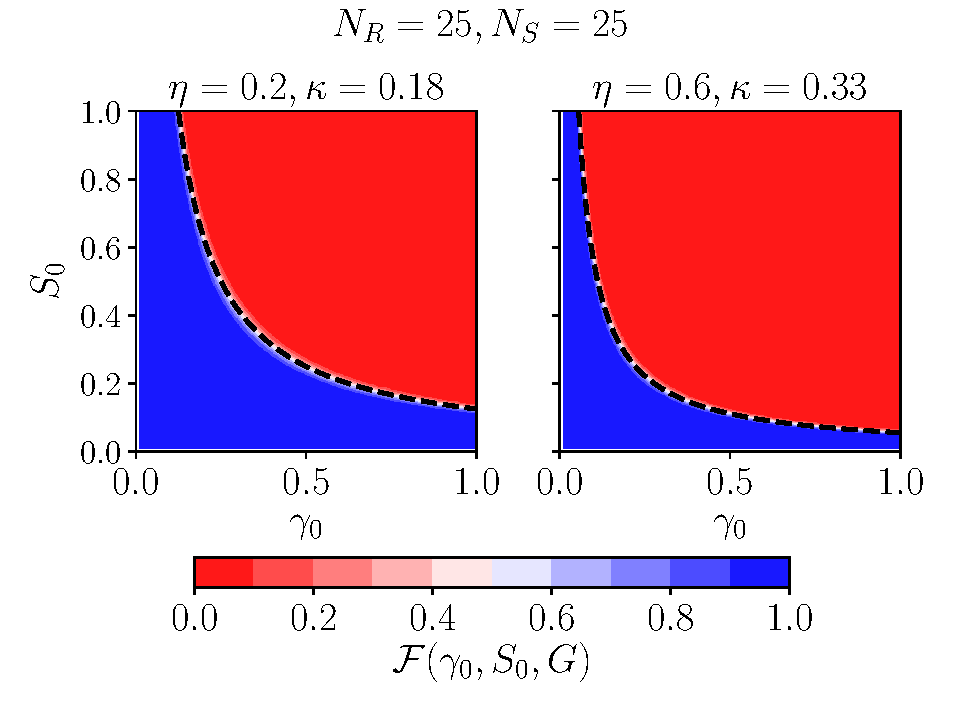
\includegraphics{Results/typical_feasibility_volume}
\caption{Plot of the feasability area. The color curve indicicates the feasibility function $\mathcal{F}$ for the matrix of our set with connectance $0.18$ and nestedness $0.15$ . We observe a steep descent from a totally feasible to totally unfeasible regime. A fit of the points $\mathcal{F}(\gamma_0, S_0) \approx 0.5 $ yields $S_0 = 0.17310809 \gamma_0 -0.0029606$
(with a relative error of $10^{-6}$). The theoretical prediction is $S_0 = 0.2 \gamma_0$. The full line indicates the theoretical critical feasibility volume, and the dashed area the measured one. Although not perfect it matches quite well. A fit yields $S_0 = 0.04261718 \gamma_0 -0.00456834$ with a relative error of the order of $10^{-6}$. Theoretical predicts $S_0=0.0526316 \gamma_0$}
\label{fig : feasability region}
\end{figure}
\end{document}
